\documentclass[xcolor=dvipsnames,8pt]{beamer}
% ********** Styl prezentacji **********
\mode<presentation>
{
%\usetheme{Frankfurt}
%\usetheme{Copenhagen}
%\usetheme{Madrid}
\usetheme{Warsaw}
%\usetheme{lankton-keynote}
 %Copenhagen
}
%\usepackage{amsmath}
%\usepackage{amsthm}
%\usepackage{amsfonts}
\usepackage{color}
%\usepackage{listings}
%\lstset{language=C++}
%\usepackage{lscape} 
%\usepackage{float}
%\usepackage{graphicx}
\usepackage{caption}
\usepackage{subcaption}
%\usepackage{multimedia}
% common reference commands
\newcommand{\eqt}[1]{Eq.~(\ref{#1})}                     % equation
\newcommand{\fig}[1]{Fig.~\ref{#1}}                      % figure
\newcommand{\tbl}[1]{Table~\ref{#1}}                     % table
%\usepackage{movie15}
%\usepackage{hyperref}
%\usepackage{multimedia}
\usepackage[]{media9}
%\usepackage{filecontents,hyperref,listings}
\renewcommand{\div}{\vec{\nabla} \cdot}
\newcommand{\grad}{\vec{\nabla}}
\newcommand{\mbold}[1]{\boldsymbol#1}
\newcommand{\tcm}[1]{\textcolor{magenta}{#1}}
\newcommand{\tcr}[1]{\textcolor{red}{#1}}
\newcommand{\tcb}[1]{\textcolor{blue}{#1}}
%
%\setbeamertemplate{footline}[frame number]
%\title{Extension of the entropy viscosity method to low Mach regime and the seven equations model.}
%\title{Extension of the entropy viscosity method to low Mach regime and the seven equations model.}
%\author{Marc-Olivier Delchini}
%
\date{09/30/2014}

%\addtobeamertemplate{footline}{\hfill\insertframenumber/\inserttotalframenumber\hspace{2em}\null}

\setbeamertemplate{footline}{
\leavevmode%
%\hbox{\hspace*{-0.06cm}
\begin{beamercolorbox}[wd=.5\paperwidth,ht=3.25ex,dp=1ex,center]{author in head/foot}%
	\usebeamerfont{author in head/foot}\insertshortauthor%~~(\insertshortinstitute)
\end{beamercolorbox}%
\begin{beamercolorbox}[wd=.25\paperwidth,ht=3.25ex,dp=1ex,center]{section in head/foot}%
	\usebeamerfont{section in head/foot} PHYSOR-2014 % \insertshorttitle
\end{beamercolorbox}%
\begin{beamercolorbox}[wd=.25\paperwidth,ht=3.25ex,dp=1ex,left]{section in head/foot}%
	\usebeamerfont{section in head/foot}\insertshortdate{}\hspace*{2em}
	\insertframenumber{} / \inserttotalframenumber %\hspace*{2ex}
\end{beamercolorbox}}%
%\vskip0pt%
%}

\beamertemplatetransparentcovered

\urldef{\ragusa}\url{jean.ragusa@tamu.edu}
\urldef{\delchini}\url{delcmo@tamu.edu}
\urldef{\berry}\url{ray.berry@inl.gov}

\title{Extension of the Entropy Viscosity Method to the Seven-Equation two-phase flow Model}

\author{Marc O. Delchini$^\star$, Jean C. Ragusa$^\star$, Ray Berry$^\ddagger$}
\institute{
$^\star$   Texas A\&M University, College Station, TX, USA\\
$^\dagger$ Idaho National Laboratory, Idaho Falls, ID, USA}
%
\begin{document}
%
\begin{frame}
%\maketitle
\titlepage
\small{email:  {\delchini}, {\ragusa}, {\berry} }
\end{frame}
%\begin{frame}
%\begin{center} ANS Winter Meeting 2014 \end{center}
%\begin{center} {\LARGE } \end{center}
%
%\begin{center} M-O. Delchini \footnote{Nuclear Engineering Department, Texas A\&M University.}, J. Ragusa$\ ^1$, 
%R. Berry \footnote{Idaho National Laboratory}.\end{center}
%\begin{center} \today \end{center}
%\end{frame}
%
\begin{frame}
	\frametitle{Outline:}
	\tableofcontents
\end{frame}
%************************************************
\section{Introduction / Background}
%************************************************
\begin{frame}{\normalsize Introduction}

\end{frame}
%************************************************
\begin{frame} 
\frametitle{\normalsize All-speed fluid flow solver}
\begin{block}{Goal}
To use \tcm{compressible} fluid equations for \tcm{all Mach} numbers\\
To solve them using \textcolor{red}{{\it continuous} FEM} using MOOSE 
\end{block}

\begin{block}{All-speed fluid flow solver}
Low-Mach: huge disparity in speeds (pressure waves move much faster)\\
\hspace{0.5cm} $\bullet$ Severely CFL-constrained if using explicit time-stepping\\
\hspace{0.5cm} $\bullet$ Best to use \tcr{implicit} time stepping \\
\hspace{0.5cm} $\bullet$ Nonlinear system of equations \\%(preconditioner: pressure-correction ICE, for example)\\
\hspace{0.5cm} $\bullet$ Fits the JFNK formalism in MOOSE where all physic components are tightly coupled \\
\end{block}

\begin{block}{Regularization technique for discretization of fluid flow}
We will employ novel artificial viscosity schemes based on the entropy production residual
{\small (Guermond et al., {\it Entropy viscosity method for nonlinear  conservation laws}, J. of Comput. Phys. (2011).}\\
\medskip
The \tcm{entropy viscosity method} is \tcr{discretization-independent} and was significantly tested in the supersonic regime
(including using \tcr{continuous FEM}).
\end{block}
\end{frame}
%************************************************
\begin{frame}{\normalsize Background}

\end{frame}
%************************************************
\section{The Seven-Equation two-phase flow Model (SEM)}
%************************************************
\begin{frame}{\normalsize The Seven-Equation two-phase flow Model (1/2)}
We consider two phases ${j,k}$. Phase $k$ obeys the following system of equations:
\begin{block}{}
\begin{subequations}
%\left\{
%\begin{array}{lcll}
Void fraction equation:
\begin{equation}
\partial_t \left( \alpha_k  A\right) + A {\color{violet}\vec{u}_{int}} \cdot \grad \alpha_k = {\color{red}\mu_{rel}} {\color{blue}A \left( P_k - P_j \right)} \nonumber 
\end{equation}
Continuity equation:
\begin{equation}
\partial_t \left( \alpha_k \rho_k A \right) + \div \left( \alpha_k \rho_k \vec{u}_k A \right) = 0 \nonumber
\end{equation}
Momentum equation:
\begin{align}
\partial_t \left( \alpha_k \rho_k \vec{u}_k A \right) +& \div \left[ \alpha_k A \left( \rho_k \vec{u}_k\otimes \vec{u}_k \right) \right]  + \grad(\alpha_k A P_k) =  \nonumber \\
&\alpha_k P_k \grad A +  {\color{violet}P_{int}} A \grad \alpha_k +  {\color{red}\lambda_{rel}}{\color{blue}A  \left( \vec{u}_j - \vec{u}_k \right)} \nonumber
\end{align}
Energy equation:
\begin{align}
\partial_t \left( \alpha_k \rho_k E_k A \right) +& \div \left[ \alpha_k A \vec{u}_j \left( \rho_k E_k + P_k \right) \right] = \nonumber \\
&A {\color{violet}P_{int} \vec{u}_{int}} \cdot \grad \alpha_k - {\color{red}\mu_{rel}} {\color{violet}\bar{P}_{int}} {\color{blue}A\left( P_k-P_j \right)} + {\color{red}\lambda_{rel}} {\color{violet}\bar{\vec{u}}_{int}} {\color{blue}A \cdot \left( \vec{u}_j - \vec{u}_k \right)} \nonumber
\end{align}
%\end{array}
%\right.
\end{subequations}
\end{block}
\end{frame}
%************************************************
\begin{frame}{\normalsize The Seven-Equation two-phase flow Model (2/2)}
\begin{block}{\normalsize Interfacial ($P_{int}$ and $\vec{u}_{int}$) and relaxation parameters ($\lambda_{rel}$ and $\mu_{rel}$)}
\begin{equation}
\left\{
\begin{array}{l}
P_{int} = \bar{P}_{int} - \frac{Z_k Z_j}{Z_k + Z_j} \frac{\grad \alpha_k}{|\grad \alpha_k|} \cdot \left( \vec{u}_k-\vec{u}_j \right) \\
\bar{P}_{int} = \frac{Z_k P_j + Z_j P_k}{Z_k + Z_j} \\
\vec{u}_{int} = \bar{\vec{u}}_{int} - \frac{\grad \alpha_k}{|\grad \alpha_k|} \frac{P_k - P_j}{Z_k + Z_j} \\
\bar{\vec{u}}_{int} = \frac{Z_k \vec{u} _k + Z_j \vec{u}_j}{Z_k + Z_j} \\
\end{array}
\right.
\nonumber
\text{ and }
\left\{
\begin{array}{l}
\mu_{rel} = \frac{A_{int}}{Z_k+Z_j} \\
\lambda_{rel} = \frac{\mu_{rel}}{2} Z_k Z_j \\
A_{int} = 6.25 \ A^{max}_{int} \ \alpha_k \left( 1-\alpha_k \right)^2
\end{array}
\right.
\end{equation}
\end{block}
\begin{block}{\normalsize Phasic entropy residual}
\begin{align}
(s_{e})_k^{-1} \alpha_k \rho_k A \frac{Ds_k}{Dt} &= \mu_{rel} \frac{Z_k}{Z_k+Z_j} (P_j - P_k)^2 + \lambda_{rel} \frac{Z_j}{Z_k+Z_j} (\vec{u}_j -\vec{u}_k)^2 \nonumber
\\
& \frac{Z_k}{\left( Z_k+Z_j \right)^2} \left[ Z_j (\vec{u}_j-\vec{u}_k)+\frac{\grad \alpha_k}{|| \grad \alpha_k ||}(P_k-P_j)\right]^2 \geq 0 \nonumber
\end{align}
\end{block}
\end{frame}
%************************************************
\section{A numerical method: the Entropy Viscosity Method (EVM)}
%************************************************
\begin{frame} 
\frametitle{\normalsize Quick overview of the entropy-based artificial viscosity formalism}

General scalar conservation law: $\partial_t u + \div \vec{f}(u) = 0$.

\begin{enumerate}
\item Determine an entropy pair ($s(u),\, \vec{\Psi}(u)$) for the PDE under consideration
\item Compute the entropy residual $R_e:=\partial_t s(u_h) + \div \Psi(u_h)$, in each cell $K$, at each quadrature point $x_q$
\item Compute the speed associated with this residual
\begin{equation}
v_e := h \frac{|R_e(x_q)|_K}{|s-\overline{s}|_\infty}
\end{equation}
%The denominator is used to normalize the residual
%. It is the deviation of $E(u)$ from the domain average $\overline{E}$.
\item Define the dynamic viscosity (m$^2$/s) as
\begin{equation}
\mu := h \min \Big( \frac{1}{2} |\vec{f}'(u)|, \, v_e \Big)
\end{equation}
\item Plug in the standard Galerkin weak form as a \tcm{viscous regularization} %(\tcm{it is really a straightforward technique})
\begin{equation}
\int_V \big( \partial_t u_h + \div \vec{f}(u_h) \big) b \, dx + \tcm{\sum_K \int_K \mu_K \grad u_h \grad b \, dx} = 0 \quad \forall b
\end{equation}
\end{enumerate}
\end{frame}
%************************************************
\begin{frame}
\frametitle{\normalsize Example: Burgers equation}
\begin{figure}
        \centering
        \begin{subfigure}[b]{0.37\textwidth}
                \centering
                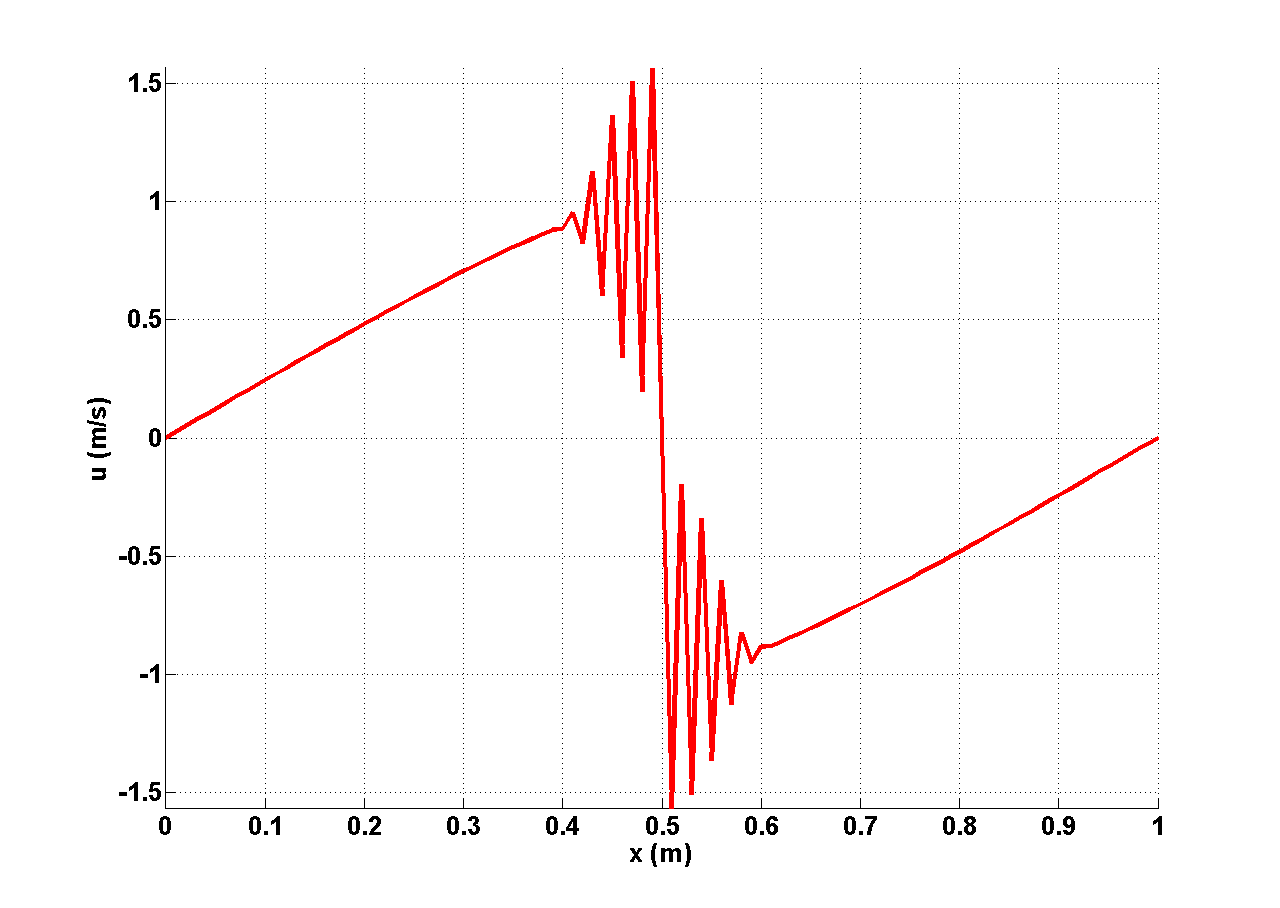
\includegraphics[width=\textwidth]{figs/1D_sol_free.png}
                \caption{Without stabilization.}
        \end{subfigure}%
        \begin{subfigure}[b]{0.37\textwidth}
                \centering
                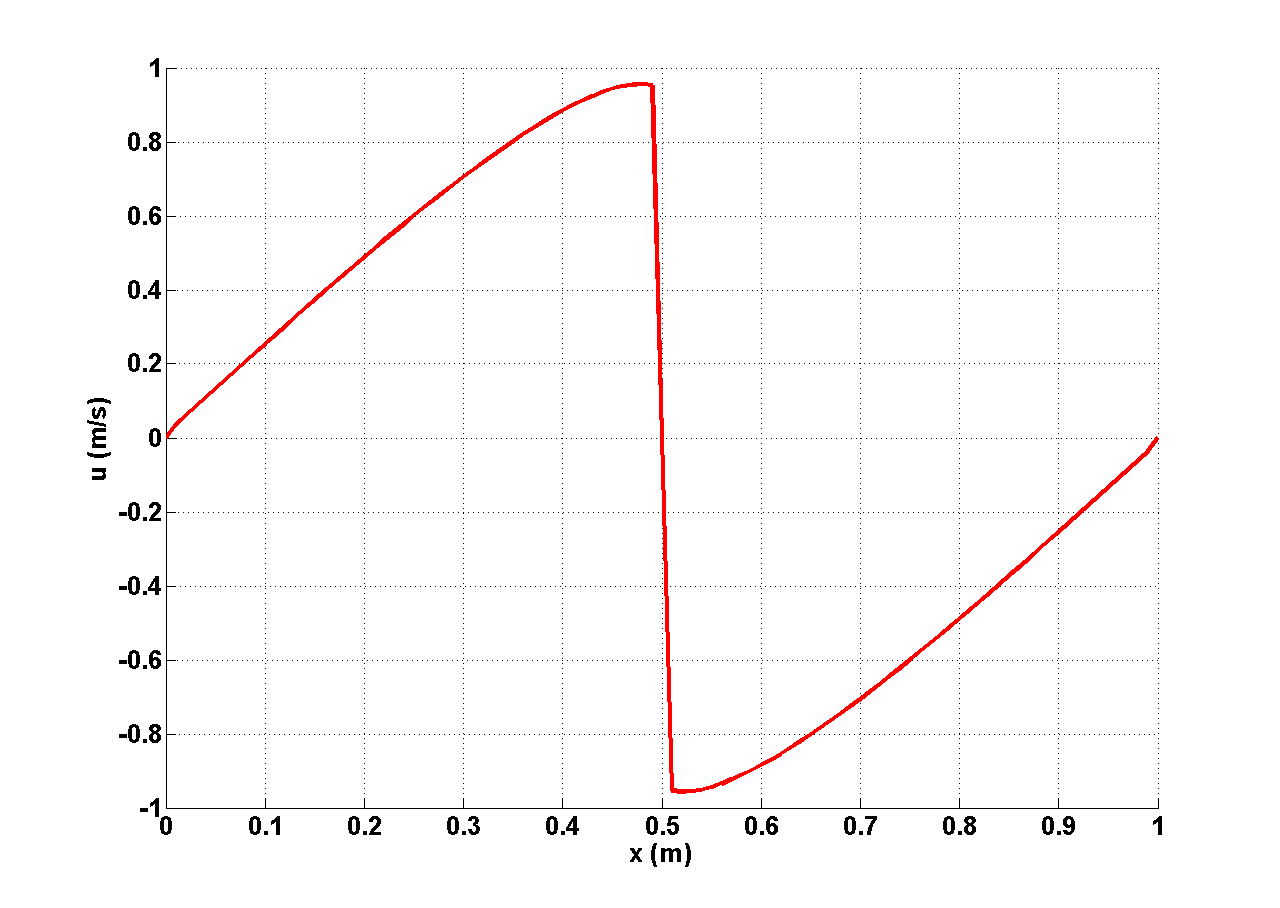
\includegraphics[width=\textwidth]{figs/1D_sol_fo.png}
                \caption{With first-order viscosity.}
        \end{subfigure}
        
        \begin{subfigure}[b]{0.37\textwidth}
                \centering
                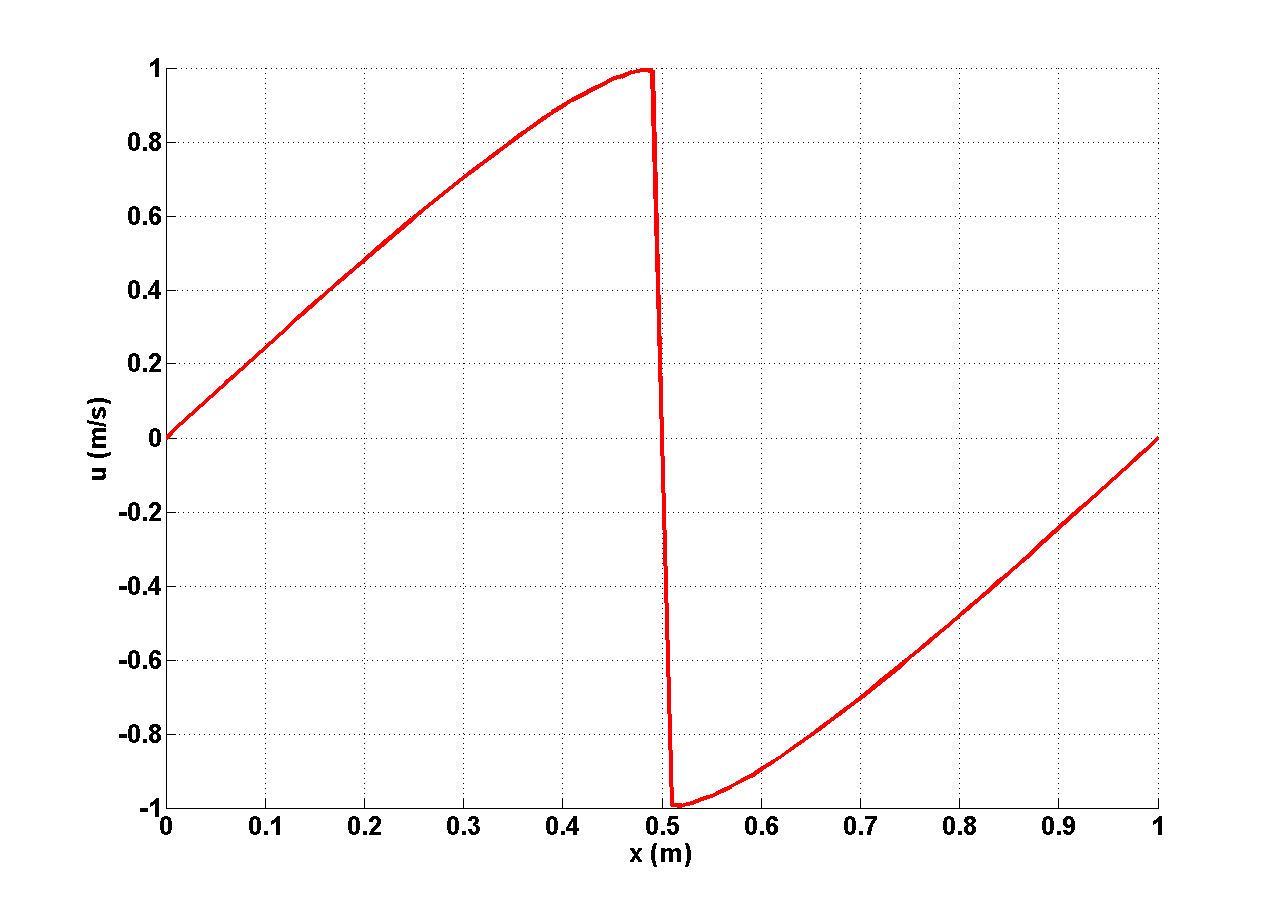
\includegraphics[width=\textwidth]{figs/1D_sol_ev.png}
                \caption{With the EVM.}
        \end{subfigure}
        \begin{subfigure}[b]{0.37\textwidth}
                \centering
                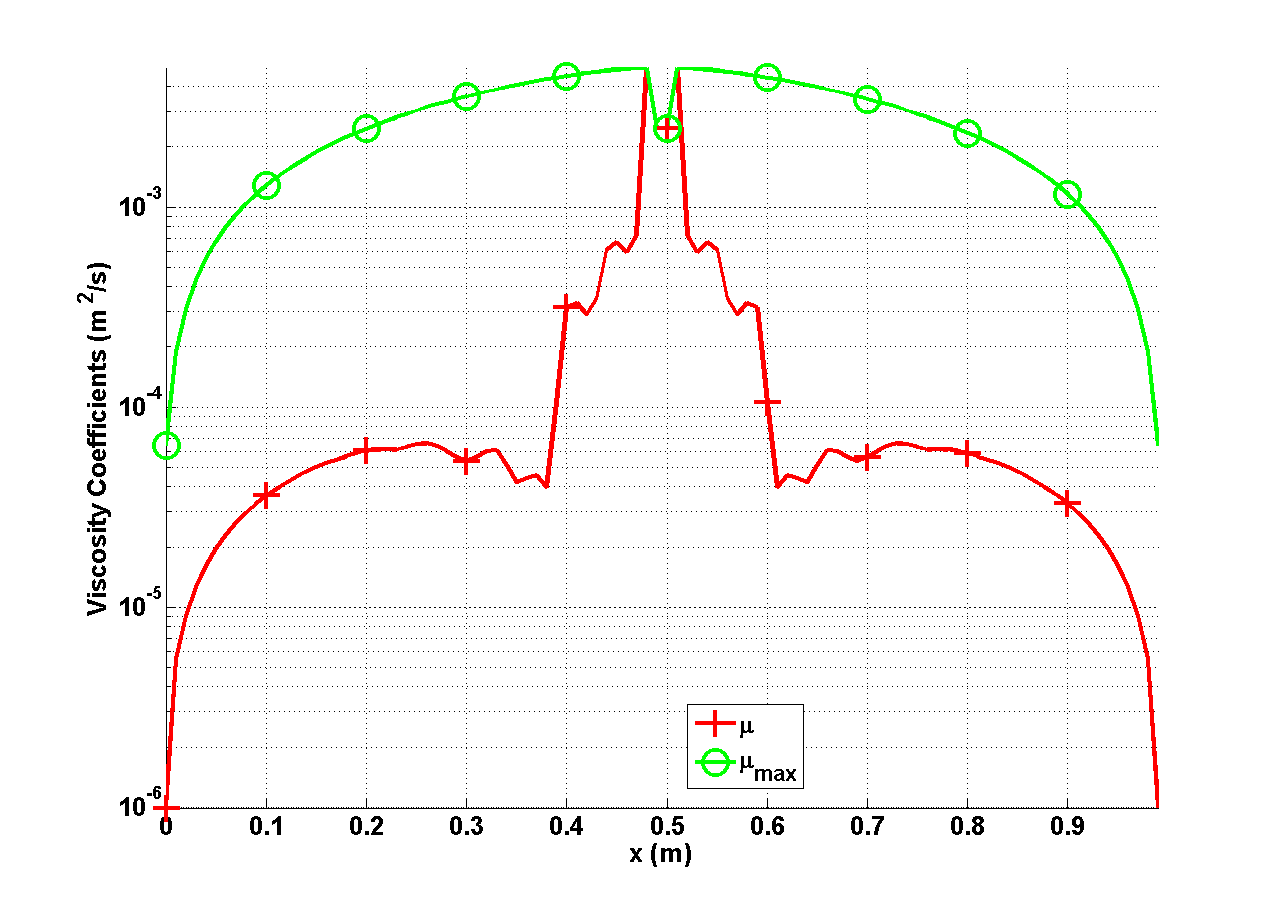
\includegraphics[width=\textwidth]{figs/1D_visc.png}
                \caption{Viscosity coefficient profiles.}
        \end{subfigure}
\end{figure}
\end{frame}
%************************************************
\section{The Entropy Viscosity Method applied to the SEM.}
%************************************************
%\begin{frame}{Low Mach regime:}
%\begin{block}{}
%{\color{red}The numerical methods developed to resolve shocks for supersonic flows are usually ill-scaled in the low Mach regime \cite{LowMach1, LowMach2, LowMach3}.} 
%\begin{itemize}
%\item The dissipative terms become dominant and change the nature of the equations.
%\item A fix is often required in the low Mach regime in order to yield the correct behavior $\rightarrow$ add enough viscosity to stabilize the scheme but not too much so that the physical solution is not altered. 
%\item Example with Roe scheme \cite{Roe}: a fix was designed in order to obtain the correct asymptotic behavior in the low Mach regime.
%\begin{equation}
%\mathbf{F}(\mathbf{U}) = (1-M) \cdot \mathbf{F}_{\text{Low Mach}}(\mathbf{U}) + M \cdot \mathbf{F}_{Roe}(\mathbf{U}) \nonumber
%\end{equation}
%\item Example of scaling analysis with artificial dissipative terms: upwind scheme.
%\begin{equation}
%\partial_{t} \rho + \div \left( \rho \vec{u} \right) = \frac{1}{2}\left( 1 + \frac{1}{M^*} \right)  \div \left(\kappa \grad \rho \right) \nonumber
%\end{equation}
%\end{itemize}
%\end{block}
%\end{frame}
%************************************************
%\subsection{RELAP-7: reactor safety analysis code.}
%\begin{frame}{RELAP-7: reactor safety analysis code.}
%\begin{block}{What is RELAP-7?}
%\begin{itemize}
%\setlength{\itemsep}{15pt}
%\item Developed by Idaho National Laboratory (INL). 
%\item $1$-D reactor analysis system.
%\item Based on the MOOSE \cite{Moose} framework (C++): fully implicit code.
%\item Safety applications for PWR, BWR and gas reactors.
%\item Solve compressible system of equations using conservative variables $(\rho, \rho \vec{u}, \rho E)$.
%\end{itemize}
%\end{block}
%\end{frame}
%************************************************
%\begin{frame}
%\begin{block}{Fluid solver requirements:}
%\begin{enumerate}
%\setlength{\itemsep}{1pt}
%\item Compressible single and two-phase flow equations.
%\item Being able to resolve shocks: numerical method.
%\item Valid for any equation of state of type $P = eos(\rho, e)$.
%\item Valid for a wide range of Mach numbers: compressible and incompressible flows.
%\item Account for source terms: wall friction, wall heat source, gravity force, $\dots$
%\item Use \emph{implicit} temporal integrators: Backward Euler and BDF2.
%\end{enumerate}
%\end{block}
%\begin{block}{The entropy viscosity method, a good candidate?}
%\begin{itemize}
%\setlength{\itemsep}{1pt}
%\item 1 and 2 are met by the entropy viscosity method ONLY for single-phase flow.
%\item 3: there exists a theoretical proof that states the method can be applied to any EOS with a convex entropy function.
%\item 4, 5 and 6 are investigated here.
%\end{itemize}
%\end{block}
%\end{frame}
%************************************************
%\subsection{The entropy viscosity method.}
%\begin{frame}{The entropy function:}
%For a given hyperbolic system of equations: $\partial_t \mathbf{U} + \div \mathbf{F} \left( \mathbf{U} \right) = 0$
%\begin{block}{Definition of the physical entropy (ref):}
%An entropy is a function that is positive and increases with time: 
%\end{block}
%\begin{block}{Entropy inequality (ref):}
%\begin{equation}
%\partial_t \mathbf{U} + \div \mathbf{F} \left( \mathbf{U} \right) = 0 \Rightarrow \partial_t s + \div \Phi (s)  \geq 0 \nonumber
%\end{equation}
%\end{block}
%\begin{block}{Example: multi-D Euler equations \cite{Toro}}
%\begin{equation}
%\partial_t s(\rho,e) + \vec{u} \cdot \grad s(\rho,e) \geq 0 \nonumber
%\end{equation}
%\end{block}
%\end{frame}
%************************************************
\begin{frame}{\normalsize The multi-D seven-equation model (with variable area) \cite{SEM}:}
\begin{block}{The model:}
\begin{itemize}
\setlength{\itemsep}{10pt}
\item Each phase obeys the single-phase Euler equations: two continuity equations, two momentum equations and two energy equations.
\item Seventh equation: void fraction equation $\rightarrow$ an internal boundary condition between the two phases at the interface.
\item Exchange terms between phases: relaxation terms. These terms were derived using \emph{rational thermodynamic} \cite{RatTherm} $\rightarrow$ consistent with the entropy minimum principle.
\item {\color{red}The system of equations is well-posed, it has 7 real eigenvalues.}
\item The seven-equation model degenerates to single-phase Euler equations when one phase disappears.
\end{itemize}
\end{block}
\end{frame}
%************************************************
%\subsubsection{Preliminary numerical results.}
%\begin{frame}{$1$-D numerical results: nozzle.}
%\centering
%$\mu_{rel}$ and $\lambda_{rel}$ $\to \infty$
%\begin{figure}[H]
%        \centering
%        \begin{subfigure}[b]{0.4\textwidth}
%                \centering
%                \includegraphics[width=\textwidth]{Sevan_pressure.png}
%%                \caption{Pressure}
%        \end{subfigure}%
%        ~ %add desired spacing between images, e. g. ~, \quad, \qquad etc. 
%          %(or a blank line to force the subfigure onto a new line)
%        \begin{subfigure}[b]{0.4\textwidth}
%                \centering
%                \includegraphics[width=\textwidth]{Sevan_velocity.png}
%%                \caption{Velocity.}
%        \end{subfigure}
%         %add desired spacing between images, e. g. ~, \quad, \qquad etc. 
%          %(or a blank line to force the subfigure onto a new line)
%        \begin{subfigure}[b]{0.4\textwidth}
%                \centering
%                \includegraphics[width=\textwidth]{Sevan_vf.png}
%%                \caption{Density.}
%        \end{subfigure}
%         \begin{subfigure}[b]{0.4\textwidth}
%                \centering
%                \includegraphics[width=\textwidth]{Sevan_viscosity.png}
%%                \caption{Viscosity coefficients.}
%        \end{subfigure}
%        \caption{Steady-state numerical solution with $100$ cells, linear polynomials and BDF2.}
%        \end{figure}
%\end{frame}
%************************************************
\section{1-D numerical results}
%************************************************
\section{Conclusions and future work}
\begin{frame}{\normalsize Conclusions and future work}
\begin{block}{Conclusions}
\begin{itemize}
\setlength{\itemsep}{15pt}
\item Derived the dissipative terms using the entropy minimum principle $\rightarrow$ valid for any equation of state under the same assumptions as for Euler equations.
\item Derived a definition for the viscosity coefficients: $\mu$, $\kappa$ and $\beta$.
\item Performed tests with a $1$-D nozzle.
\end{itemize}
\end{block}
\begin{block}{Future work}
\begin{itemize}
\setlength{\itemsep}{15pt}
\item Perform some more tests in $1$-D: include mass and heat transfer between phases \cite{SEM}.
\item Tests in $2$-D.
\end{itemize}
\end{block}
\end{frame}
%************************************************
\begin{frame}{}
\begin{center}
\LARGE{\textbf{QUESTIONS/COMMENTS ?}}
\end{center}
\end{frame}
%************************************************
%************************************************
%************************************************
%************************************************
%************************************************
%************************************************
%************************************************
%************************************************
%\bibliographystyle{ans}
%\bibliography{mybibfile}
\begin{frame}[allowframebreaks]
\bibliographystyle{apalike}
\bibliography{Biblio-Database}
\begin{thebibliography}{47}
  
  \bibitem{jlg1}
  {\em Entropy viscosity method for nonlinear conservation laws}, 
  Jean-Luc Guermond, R. Pasquetti, B. Popov, J. Comput. Phys., 230 (2011) 4248-4267.
  
  \bibitem{jlg2}
  {\em Entropy Viscosity Method for High-Order Approximations of Conservation Laws}, 
  J-L. Guermond, R. Pasquetti, 
  Lecture Notes in Computational Science and Engineering, Springer, Volume 76, (2011) 411-418.

 \bibitem{jlg3}
 \emph{Entropy-based nonlinear viscosity for Fourrier approximations of conservation laws}, 
 J.-L. Guermond, R. Pasquetti, C.R. Math. Acad. Sci. Paris 346 (2008) 801�806.

  \bibitem{Neumann}
  \emph{A method for the numerical calculation of hydrodynamic shocks}, 
  J. von Neumann, R.D. Richtmyer, J. Appl. Phys. 21 (1950) 232�237
  
  \bibitem{Balsara}
  \emph{An Analysis of the Hyperbolic Nature of the Equations of Radiation Hydrodynamics},
  Dinshaw S. Balsara, J. Quant. Spectrosc. Radiat. Transfer, Vol. 61, No. 5, pp. 617-627, 1999.
  
  \bibitem{LowrieMorelHittinger}
  \emph{The coupling of radiation and hydrodynamics},
  Lowrie RB, Morel JE, Hittinger JA, 521 (1), 432-50 (1999).

  \bibitem{FluxLimiter1}
  \emph{Advanced numerical approximation of nonlinear hyperbolic equations}, 
  B. Cockburn, C. Johnson, C. Shu, E. Tadmor, Lecture Notes in Mathematics, vol. 1697, Springer, 1998.
  
  \bibitem{FluxLimiter2}
  \emph{Discontinuous Galerkin methods: theory, computation and applications}, 
  B. Cockburn, G. Karniadakis, C. Shu, Lecture Notes in Computer Science and Engineering, vol. 11, Springer, 2000.
  
  \bibitem{FluxLimiter3}
  \emph{The local discontinuous Galerkin method for time- dependent convection-diffusion systems}, 
  B. Cockburn, C. Shu, SIAM J. Numer. Anal. 35 (1998) 2440�2463.
  
\bibitem{FluxLimiter4}
\emph{New non-oscillatory central schemes on unstructured triangulations for hyperbolic systems of conservation laws}, 
I. Christov, B. Popov, J. Comput. Phys. 227 (11) (2008) 5736�5757.

\bibitem{SUPG}
\emph{Streamline upwind/Petrov-Galerkin formulations for convection dominated flows with particular emphasis on the incompressible Navier-Stokes equations},
A.N. Brooks, T.J.R. Hughes, Comput. Meths. Appl. Mech. Engrg., 32 (1982), pp. 199�259.

\bibitem{EdwardsMorelKnoll}
 \emph{Nonlinear variants of the TR$-$BDF$2$ method for thermal radiative diffusion},
 Jarrods D. Edwards, Jim E. Morel, Dana A. Knoll, Journal of Computational Physics, 230 (2011), 1198-1214.
 
  \bibitem{Toro}
  \emph{Riemann Solvers and numerical methods for fluid dynamics.}
  E.F. Toro, $2^{nd}$ Edition, Springer.  
  
  \bibitem{Reisner}
  \emph{A space-time smooth artificial viscosity method for nonlinear conservation laws}
  Reisner J., Serencsa J. and Shkoller S., Journal of Computational Physics 235 (2013) 912-933.
    
  \bibitem{valentin}
  \emph{Implementation of the entropy viscosity method with the discontinuous Galerkin method},
  Valentin Zingan, Jean-Luc Guermond, Jim Morel, Bojan Popov, Volume 253, 1 January 2013, Pages 479-490
    
  \bibitem{LowrieMorel}
  \emph{Issues with high-resolution Godunov methods for radiation hydrodynamics},
  R.B. Lowrie, J.E. Morel, Journal of Quantitative Spectroscopy \& Radiative Transfer, 69, 475-489 (2001).

\bibitem{EdwardsMorelLowrie}
\emph{Second-Order Discretization in Space and Time for Radiation Hydrodynamics},
Jarrod D. Edwards, Jim E. Morel, Robert B. Lowrie, International Conference on Mathematics and Computational Methods Applied to Nuclear Science \& Engineering (M\&C 2013), Sun Valley, Idaho USA, May 5-9, American Nuclear Society, LaGrange Park, II (2013).
   
  \bibitem{ShiJin}
  \emph{Numerical Schemes for Hyperbolic Conservation Laws with Stiff Relaxation Terms}, 
  Shi Jin and C. David Levermore, Journal of Computational Physics, 126, 449-467 (1996).
  
  \bibitem{jlg}
  \emph{Viscous regularization of the Euler equations and entropy principles},
  Jean-Luc Guermond and Bojan Popov, under review.
  
  \bibitem{Moose}
  \emph{A parallel computational framework for coupled systems of nonlinear equations},
  D. Gaston, C. Newsman, G. Hansen and D. Lebrun-Grandie, Nucl. Eng. Design, vol 239, pp 1768-1778, 2009.
  
  \bibitem{Sodov}
  \emph{Similarity and dimensional methods in mechanics},
  Sedov LI., New York: Academic Press, 1959.
  
  \bibitem{RatTherm}
  \emph{Rational thermodynamics},
  Truesdell C. and Wang C.-C., New York, McGraw-Hill Book Company, 1969, XII. 208 S.
  
  \bibitem{IGEOS}
  \emph{A to Z of Thermodynamics},
  Perrot P., Oxford University Press (1998).
  
  \bibitem{SGEOS}
  \emph{Elaborating equation of state for a liquid and its vapor for two-phase flow models.}
  O. LeMetayer, J. Massoni, R. Saurel, International Journal of Thermal Science 43 (2004) 265-276.

  \bibitem{Lapidus_paper}
  \emph{A detached shock calculation by second order finite differences},
  Lapidus A., J. Comput. Phys., 2, 154-177.

  \bibitem{LMP}
  \emph{A simple extension to multidimensional problems of the artificial viscosity due to Lapidus},
  Lohner R., Morgan K. and Peraire J., Commun. Numer. Methods Eng., 1(14), 141-147.
      
  \bibitem{Lapidus_book}
  \emph{Finite Element Methods for Flow Problems},
  Jean Donea and Antonio Huerta, 2003,  Edition, Wiley.
  
  \bibitem{PBV_book}
  \emph{Applied CFD Techniques: an Introduction based on Finite Element Methods},
  Rainald Lohner, $2^{nd}$ Edition, Wiley.
  
  \bibitem{Roe}
  \emph{An All-Speed Roe-type scheme and its asymptotic analysis of low Mach number behavior},
  Xue-song Li, Chun-wei Gu, Journal of Computational Physics 227 (2008) 5144-5159
  
  \bibitem{LowMach1}
  \emph{On the behavior of upwind schemes in the low Mach number limit},
  Guillard H., Viozat C., Computers \& Fluids 28 (1999) 63-86.
  
  \bibitem{LowMach2}
  \emph{Preconditioned techniques in computational fluid dynamics.}
  E.Turkel, Annu. Rev. Fluid Mech. (1999) 31:385-416.  
  
  \bibitem{LowMach3}
  \emph{The solution of the compressible Euler equations at low Mach numbers using a stabilized finite element algorithm},
  J. S. Wong, D.L. Darmofal, J. Peraire, Comput. Methods Appl. Mech. Engrg. 190 (2001) 5719-5737.
  
  \bibitem{SEM}
  \emph{The discrete equation method (DEM) for fully compressible, two-phase flows in ducts of spatially varying cross-section.}
  R. Berry, R. Saurel, O. LeMetayer,
  Nuclear Engineering and Design, 240 (2010) 3797-3818.
  
  \bibitem{Riemann12}
  \emph{Comparison of several difference schemes on 1D and 2D test problems for the Euler equations}, 
  R. Liska, B. Wendroff, SIAM J. Sci. Comput. 25 (3) (2003) 995� 1017 (electronic).
  
  \bibitem{Mach3Step}
  \emph{An evaluation of several differencing methods for inviscid fluid flow problems}, 
  A.F. Emery, J. Comput. Phys. 2 (1968) 306�331.
  
  \bibitem{CompressionCorner}
  \emph{Modern Compressible Flow}, 
  Anderson, J.D. (1982), McGraw Hill Inc., New York. ASME (2006). V\&V 10-2006 Guide for Verification and Validation in Computational Solid
Mechanic.
  
  \bibitem{Hump}
  \emph{A Robust Multigrid Algorithm for the Euler Equations with Local Preconditioning and Semi-coarsening},
  D. L. Darmofal and K. Siu, Journal of Computational Physics 151, 728�756 (1999).
  
  \bibitem{Leblanc}
  \emph{Validation Test Case Suite for compressible hydrodynamics computation},
  Loubere R., Theoritical Division, T-7, Los Alamos National Laboratory (pdf version).
  
  \bibitem{ShockTEOS}
  \emph{A New Averaging Scheme for the Riemann Problem in Pure Water},
  Tze-Jang Chen, C. H. Cooke, Mathl. Comput. Modeling Vol. 25 No. 3, pp. 25-36, 1997.
\end{thebibliography}
\end{frame}
%************************************************
%************************************************
%************************************************
%************************************************
%************************************************
%************************************************
%************************************************
%************************************************
%\begin{frame}{Viscous regularization for the multi-D seven-equation model:}
%\begin{equation}
%\left\{
%\begin{array}{lll}
%\partial_t \left( \alpha_k  A\right) &+ \vec{u}_{int} A \grad \alpha_k = {\color{blue}A \mu_{rel} \left( P_k - P_j \right)} + {\color{red}\div \vec{l}} & \nonumber \\
%\partial_t \left( \alpha_k \rho_k A \right) &+ \div \left( \alpha_k \rho_k \vec{u}_k A \right) = {\color{red}\div \vec{f}}& \nonumber \\
%\partial_t \left( \alpha_k \rho_k \vec{u}_k A \right) &+ \div \left[ \alpha_k A \left( \rho_k \vec{u}_k\otimes \vec{u}_k \right) \right]  + \grad(\alpha_k A P_k) =  \nonumber \\
%&\alpha_k P_k \grad A +  P_{int} A \grad \alpha_k +  {\color{blue}A \lambda_{rel} \left( \vec{u}_j - \vec{u}_k \right)} +{\color{red}\div \bar{g}}&\nonumber \\
%\partial_t \left( \alpha_k \rho_k E_k A \right) &+ \div \left[ \alpha_k A \vec{u}_j \left( \rho_k E_k + P_k \right) \right] =& \\
% &P_{int} \vec{u}_{int} A \grad \alpha_k - {\color{blue}\mu_{rel} \bar{P_{int}} \left( P_k-P_j \right)} +{\color{blue}\bar{\vec{u}}_kA \lambda_{rel} \left( \vec{u}_j - \vec{u}_k \right)} + {\color{red}\div \vec{h}}& \nonumber
%\end{array}
%\right.
%\end{equation}
%\begin{equation}
%\left\{
%\begin{array}{lcl}
%{\color{red}\vec{l}} = A {\color{magenta}\beta_k} \grad \alpha_k & & \\
%{\color{red}\vec{f}} = \alpha_k A {\color{magenta}\kappa_k}  \grad \rho_k + \rho_k \vec{l}& & \\
%{\color{red}\bar{g}} = \alpha_k A \rho_k {\color{magenta}\mu_k} \grad \vec{u} + \vec{u} \otimes \vec{f} & & \\
%{\color{red}\vec{h}} = \alpha_k A {\color{magenta}\kappa_k} \grad(\rho_k e_k) - \frac{||\vec{u}||^2}{2} \vec{f} + \vec{u} \cdot \bar{g} + \rho_k e_k \vec{l} & &
%\end{array}
%\right.
%\nonumber
%\end{equation}
%Entropy equation:
%\begin{eqnarray}
%\alpha_k A \rho_k \frac{ds_k}{dt} + \left( {\color{green}\alpha_k A \rho_k \kappa_k} + {\color{red}\rho_k l_k} \right) \grad s_k - {\color{green}\div \left( \alpha_k A \rho_k \grad s_k \right)} = \nonumber \\ {\color{green}\partial_e s_k \alpha_k A \rho_k \mu_k \grad^s \vec{u} :  \grad \vec{u}}- {\color{green}X_k \Sigma_k X_k^t} + {\color{blue}Q}
%\nonumber
%\end{eqnarray}
%\end{frame}
%************************************************
\end{document}

